\def\vect#1,#2{\left(\!\!\!\begin{array}{c}#1\\#2\end{array}\!\!\!\right)}
\newcommand{\mvect}[1]{\left(\!\!\!\begin{array}{c}#1%
\end{array}\!\!\!\right)}

\chapter{Vektoren}
	
	Autor: Gerhard Gossen
	
\noindent	\"Uberarbeitung: Marko Rak, Melanie Pflaume
	
	\section{Definition}
	
		Der Vektor \[\overrightarrow{
        x
        }
         = \mvect{ x_1\\ x_2 \\ \vdots \\ x_n}\] ist
		ein $n$-dimensionaler Vektor. Die \emph{Komponenten} $x_1, x_2,
		\dots, x_n$ sind reelle Zahlen. In der Vorlesung wird statt
		$\overrightarrow{x}$ meist nur $x$ geschrieben.
		
		\noindent Geometrisch interessant sind Vektoren der Dimension 2 \[x =
		\mvect{x\\y} \text{ und Dimension 3: } x = \mvect{x\\y\\z}.\] Sie können als
		Pfeile in
		eine bestimmte Richtung dargestellt werden. Man kann sie auch als
		\emph{Verschiebung} interpretieren.
		Der Nullvektor $\overrightarrow0$ bzw. $0$ ist der Vektor, bei dem alle
		Komponenten $0$ sind.
		Der \emph{Ortsvektor} eines Punktes $P$ ist der Vektor 
		zwischen dem Ursprung des Koordinatensystems und $P$.
		Ein \emph{Skalar} ist eine einzelne Zahl vom selben Typ wie $x_1, x_2, \dots,
		x_n$.
		
		\begin{center}
			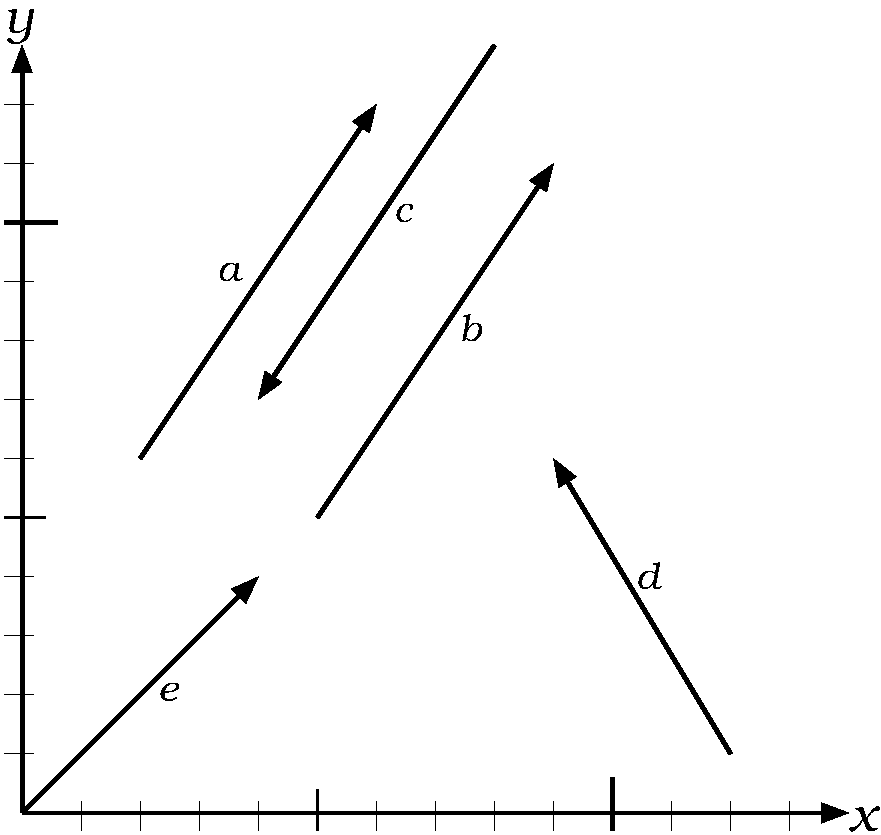
\includegraphics[width=.3\textwidth]{img/vektoren.pdf}
			
			{\scriptsize$a = \vect4,6 = b,\ c = \vect-4,{-6}=-1\cdot a,\ d= \vect{-3},5,\
			e=\vect4,4$}
		\end{center}
	
	\section{Operationen}
	
		\subsection{Addition und Subtraktion}
			Zwei Vektoren werden addiert, indem die einzelnen Komponenten addiert werden:	
			\[x + y = \mvect{x_1 \\ x_2 \\ \vdots \\ x_n} +
			\mvect{y_1 \\ y_2 \\ \vdots \\ y_n} = \mvect{x_1 + y_1 \\ x_2 + y_2 \\ \vdots
			\\ x_n + y_n}\]
		
			Die Subtraktion ist analog:
			\[x - y = \mvect{x_1 \\ x_2 \\ \vdots \\ x_n} - \mvect{y_1 \\ y_2 \\ \vdots \\
			y_n} = \mvect{x_1 - y_1 \\ x_2 - y_2 \\ \vdots \\ x_n - y_n}\]
			
			Beispiele:
			\[\hspace{-6.23pt}
            \begin{array}{ccc}
				\mvect{2\\4}+\mvect{6\\7} = \mvect{8\\11}  &\mvect{3\\7}+\mvect{0\\0}
				= \mvect{3\\7} & \mvect{1\\2\\3}+\mvect{4\\5\\6}=\mvect{5\\7\\9}\\
				\mvect{2\\4}-\mvect{6\\7} = \mvect{-4\\-3} &\mvect{3\\7}-\mvect{0\\0}
				= \mvect{3\\7} & \mvect{12\\-5\\0}-\mvect{-7\\4\\3}=\mvect{19\\-9\\-3}
			\end{array}\]
			
			\noindent Geometrisch gesehen entspricht die Addition der Vektoren $a$ und $b$
			der Verschiebung, die durch Verschieben zuerst in Richtung $a$ und danach in
			Richtung $b$ entsteht. Wie man in der Zeichnung erkennt, ist die Addition
			\emph{kommutativ}, d.\,h. $a+b = b+a$.
			\begin{center}
				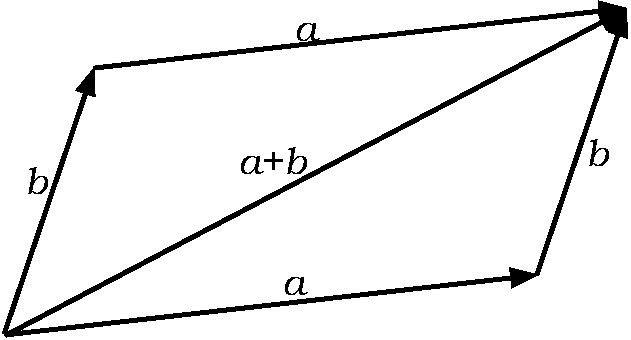
\includegraphics[height=2cm]{img/vektor_addition} 
			\end{center}
	
		\subsection{Multiplikation mit einem Skalar}
			Ein Vektor wird mit einem Skalar multipliziert, indem jede einzelne
			Komponente mit dem Skalar multipliziert wird:
			\[\lambda\cdot x = \lambda\cdot \mvect{x_1 \\ x_2 \\ \vdots \\ x_n} =
			\mvect{\lambda\cdot x_1 \\ \lambda\cdot x_2 \\ \vdots \\ \lambda\cdot x_n}\]
			Die Multiplikation mit dem Skalar $0$ ergibt immer den Nullvektor.
			
			Beispiele:
			\[\hspace{-15.14pt}\begin{array}{cccc}
				 1\cdot\mvect{3\\6\\4}=\mvect{3\\6\\4} & 2\cdot\mvect{1\\2\\3}=\mvect{2\\4\\6} &
				 -1\cdot\mvect{3\\-3\\3} = \mvect{-3\\3\\-3} &
                 0\cdot
				\mvect{3\\5\\1}=\mvect{0\\0\\0}
			\end{array}\]
			
			Geometrisch entspricht die Multiplikation einer \emph{Streckung} um den
			Faktor $\lambda$.
			
			\begin{center}
				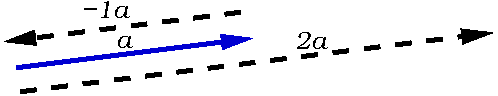
\includegraphics[width=.4\textwidth]{img/vektor_mult.pdf}
				
				{\scriptsize Vektor $a$, skaliert mit $\lambda = -1$ (oben) und $\lambda = 2$
				(unten).}
			\end{center}
	
	\section{Linearkombination}
		
		Jeder Vektor $b$, der sich als Summe $b = \lambda_1 a_1 + \lambda_2 a_2 +
		\dots + \lambda_n a_n$ darstellen lässt, heißt \emph{Linearkombination} der
		Vektoren $a_1, a_2, \dots, a_n$. Die $\lambda_i$ sind reelle Zahlen.
		
	\section{Lineare Abhängigkeit}
	
		Die Vektoren $a_1, \dots a_n$ sind \emph{linear unabhängig}, wenn die
		Gleichung 
		\[\lambda_1 a_1 + \lambda_2 a_2 + \dots + \lambda_n a_n = \overrightarrow 0\]
		nur die triviale Lösung $\lambda_1 = \lambda_2 = \dots = \lambda_n = 0$ hat. Ansonsten
		sind die Vektoren \emph{linear abhängig}.
		
		\noindent Wenn zwei oder mehr Vektoren linear abhängig sind, so kann ein Vektor als
		Linearkombination der anderen Vektoren dargestellt werden.
		
		\noindent Beispiel:
		Die Vektoren \[\mvect{2\\5\\1},\mvect{6\\2\\8},\mvect{5\\6\\5}\] sind linear
		abhängig, da \[1 \cdot \mvect{2\\5\\1} + \frac{1}{2} \cdot \mvect{6\\2\\8} =
		\mvect{5\\6\\5} \text{ bzw. } 1 \cdot \mvect{2\\5\\1} + \frac{1}{2} \cdot
		\mvect{6\\2\\8} + (-1) \cdot \mvect{5\\6\\5} = 0.\]
		
	\section{Betrag eines Vektors}
		
		Der Betrag $|a|$ eines Vektors entspricht der Länge dieses Vektors. Er wird
		berechnet als \[|a| = \left| \mvect{a_1\\ \vdots \\ a_n} \right| =
		\sqrt{\sum_{i=1}^n a_i^2}\] 
		
		Beispiele:
		\begin{align*}
			\left| \mvect{1\\0}\right| &= \sqrt{1^2+0^2} = \sqrt{1} = 1\\
			\left| \mvect{3\\4}\right| &= \sqrt{3^2+4^2} = \sqrt{25} = 5\\
			\left|\mvect{2\\-3\\1\\7\\-1}\right| &= \sqrt{2^2+(-3)^2+1^2+7^2+1^2} =
			\sqrt{4+9+1+49+1} = \sqrt{64} = 8
		\end{align*}
        
        Manchmal wird der Betrag auch anders definiert.
		
	\section{Skalarprodukt}
		Das Skalarprodukt $(a,b)$  der beiden Vektoren $a$ und $b$
		ist die reelle Zahl \[(a,b) =|a||b|\cos\alpha,\] wobei $\alpha$ der Winkel
		zwischen den
		Vektoren ist (andere Schreibweise: $a\cdot b$).
		
		\noindent Durch Umstellen entsteht eine Formel zur Bestimmung des Winkels $\alpha$:
		\begin{align*}
\cos\alpha &= \frac{(a,b)}{|a| |b|} = \frac{a_1b_1+a_2b_2+\dots
		a_nb_n}{\sqrt{a_1^2+a_2^2+\dots a_n^2}\sqrt{b_1^2+b_2^2+\dots b_n^2}} \\&
		\left( = \frac{\sum_{i=1}^n a_ib_i}{\sqrt{\sum_{i=1}^n a_i^2}\ 
		\sqrt{\sum_{i=1}^n b_i^2} } \right)\end{align*}
		
		\noindent Meist will man überprüfen, ob zwei Vektoren orthogonal zueinander sind. Mit \\
		$\cos(90^\circ) = \cos(\frac{\pi}{2}) = 0$ ergibt sich:
		\begin{equation*}
			\frac{(a,b)}{|a||b|} = 0
		\end{equation*}
	\newpage
		Beispiele:
		\begin{enumerate}
			\item Winkel zwischen $\vect1,0$ und $\vect0,1$:
			\begin{align*}
				\cos\alpha &=
				\frac{\left(\vect1,0,\vect0,1\right)}{\left|\vect1,0\right|\left|\vect0,
				1\right| }
				= \frac{1\cdot0+0\cdot1}{1\cdot1} = 0\\
				\alpha &= \arccos(0) = \frac{\pi}{2} = 90^\circ 
			\end{align*}
			
			\item Winkel zwischen $a= \mvect{-4\\2\\-2}$ und $b=\mvect{10\\-5\\5}$
			\begin{align*}
				\cos\alpha &= \frac{\left(a, b\right)}{|a||b|}\\
				            &= \frac{-40+(-10)+(-10)}{\sqrt{24}\sqrt{150}} 
				            = \frac{-60}{\sqrt{4\cdot6}\sqrt{25\cdot6}} \\
				            &= -\frac{60}{2\sqrt{6}\cdot 5\sqrt{6}} = -\frac{60}{60} = -1\\
				\alpha      &= \arccos(-1) = \pi = 180^\circ
			\end{align*}
	
		\end{enumerate}
		
		\textbf{Hinweis:}
		
		 Das Skalarprodukt zweier Vektoren n'ter Ordnung lässt sich auch folgendermaßen berechnen:\\
		\[ (\left( \begin{array}{l}
				x_{1} \\
				x_{2} \\
				\vdots \\
				x_{n}				
			\end{array} \right) ,
			\left( \begin{array}{l}
				y_{1} \\
				y_{2} \\
				\vdots \\
				y_{n}				
			\end{array} \right) )
			=
			\sum_{i=1}^{n} x_{i} \cdot y_{i}
		\]
	
	\section{Kreuzprodukt}
	
		Das \emph{Kreuzprodukt} zweier Vektoren $a$ und $b$ (beide ungleich dem
		Nullvektor) ist ein neuer Vektor. Dieser ist orthogonal zu $a$ und $b$.
		Schreibweise: $a \times b$.
		
		\noindent Das Kreuzprodukt für 3-dimensionale Vektoren wird so berechnet:
		\[a\times b = \mvect{a_1\\a_2\\a_3}\times \mvect{b_1\\b_2\\b_3} =
		\mvect{a_2b_3 - a_3b_2\\ a_3b_1 - a_1b_3\\ a_1b_2 - a_2b_1}\]
		\newline
		
		\noindent Merkhilfe: Der Wert an der Stelle $\bullet$ ergibt sich aus
		$(1)\cdot(2)-(3)\cdot(4)$, wobei $(1),\dots, (4)$ aus der Formel zu entnehmen
		sind.
		\[\hspace{-7pt}\mvect{\bullet\\\phantom{c_2} \\ \phantom{c_3}} =
		\mvect{\phantom{a_1}\\1\\3}\times
		\mvect{\phantom{b_1}\\4\\2} \quad \mvect{\phantom{c_2} \\ \bullet\\
		\phantom{c_3}} =
		\mvect{3\\\phantom{a_1}\\1}\times
		\mvect{2\\\phantom{b_1}\\4}
		 \quad \mvect{\phantom{c_2} \\ \phantom{c_3}\\ \bullet} =
		\mvect{1\\3\\\phantom{a_1}}\times
		\mvect{4\\2\\\phantom{b_1}}\]
		\newline
		Beispiele:
		\begin{align*}
			\mvect{1\\2\\3}\times \mvect{4\\5\\6} &= \mvect{2\cdot 6-3\cdot 5\\ 3\cdot 4
			- 1\cdot 6\\ 1\cdot 5 - 2\cdot 4} = \mvect{-3\\ 6 \\ -3} \\
			\mvect{1\\0\\0} \times \mvect{0\\ 1 \\ 0} &= \mvect{0\cdot0 - 0\cdot1\\
			0\cdot0 - 1\cdot 0\\ 1\cdot1 - 0\cdot0} = \mvect{0\\0\\1}
		\end{align*}
	
	\section{Literatur}
		
		Frank, Schulz, Tietz, Warmuth: \textit{Wissenspeicher Mathematik}. 1. Auflg.
		1998. Volk und Wissen Verlag Berlin. 
		
	\section{Aufgaben}
		
		\begin{enumerate}
			\item Berechne die Vektoren, mit \[a = \mvect{2\\3\\-1}, b= \mvect{-4\\1\\5},
			c = \mvect{-2\\-2\\-2}, d = \mvect{7\\9\\1}:\]
				\begin{multicols}{2}
					\begin{enumerate}
					   \item $a+b-c+d$
					   \item $d-c-b-a$
					   \item $3a-2b+c$
					   \item $a-\frac{1}{2}c+(-3)b+2d$
					   \item $2a-b+5c-d$
					   \item $3a-5b+4c+2d$
			  		\end{enumerate}
				\end{multicols}
			\item Berechne die Länge der Vektoren:
			\begin{multicols}{3}
				\begin{enumerate}
				    \item $\mvect{0\\1\\0}$
				    \item $\mvect{2\\3\\2}$
				    \item $\mvect{4\\3\\5}$
				    \item $\mvect{-2\\2\\1}$
				    \item $\mvect{3\\-3}$
				    \item $\mvect{2\\-2\\2\\2}$
				\end{enumerate}
			\end{multicols}
			\item Bestimme das Skalarprodukt der Vektoren:
			\begin{multicols}{3}
				\begin{enumerate}
				    \item $\mvect{0\\0\\1},\mvect{0\\1\\0}$
				    \item $\mvect{2\\-1\\-3}, \mvect{-2\\1\\3}$
				    \item $\mvect{3\\4\\2},\mvect{2\\-7\\5}$
			    \end{enumerate}
			\end{multicols}
			\item Bestimme den eingeschlossenen Winkel:
			\begin{multicols}{2}
				\begin{enumerate}
			    	\item $\mvect{1\\1\\0},\mvect{0\\\sqrt{2}\\0}$
			    	\item $\mvect{3\\2\\1},\mvect{-5\\1\\13}$
			    \end{enumerate}
			\end{multicols}
       
			\item Berechne das Kreuzprodukt:
				\begin{multicols}{3}
			    	\begin{enumerate}
			        	\item $\mvect{2\\5\\3}\times\mvect{-1\\2\\2}$
			        	\item $\mvect{1\\0\\2}\times\mvect{3\\4\\7}$
			        	\item $\mvect{-2\\-3\\-1}\times\mvect{-4\\-2\\-7} $
			      	\end{enumerate}
			    \end{multicols}
			\item Überprüfe, ob die Vektoren linear abhängig sind. In diesem Fall stelle
			einen der Vektoren als Linearkombination der anderen dar. (Hinweis: Nutze den Gauss-Algorithmus)
			\begin{multicols}{2}
				\begin{enumerate}
					\item $\vect1,0 , \vect1,1$
				    \item $\vect3,5 , \vect5,3$
				    \item $\vect1,2 , \vect7,3 , \vect17,5$
				    \item $\mvect{1\\0\\0}, \mvect{2\\5\\0}, \mvect{3\\7\\1}$
				    \item $\mvect{7\\2\\5}, \mvect{3\\-5\\8}, \mvect{10\\-3\\13}$
				    \item $\mvect{-2\\-3\\4}, \mvect{1\\0\\1}, \mvect{7\\6\\5}$
				    \item $\mvect{3\\7\\5}, \mvect{-2\\5\\1}, \mvect{-7\\3\\-3}$
				    \item $\mvect{1\\0\\1\\1}, \mvect{0\\1\\1\\1}, \mvect{0\\1\\3\\2},
					\mvect{1\\1\\0\\1}$
				    \item $\mvect{1\\0\\2\\1}, \mvect{1\\0\\1\\1},
					\mvect{0\\1\\0\\1}, \mvect{0\\0\\1\\1}$
				\end{enumerate}
			\end{multicols}
		\end{enumerate}